% status: 100
% chapter: Edge Computing


\def\paperstatus{100} % a number from 0-100 indicating your status. 100
                % means completed
\def\paperchapter{Edge Computing} % This section is typically a single 
                   % keyword. from a small list. Consult with theinstructors 
                   % about yours. They typically fill it out once your first
                   % text has been reviewed.
\def\hid{hid-sp18-711} % all hids of the authors of this
                                % paper. The paper must only be in one
                                % authors directory and all other
                                % authors contribute to it in that
                                % directory. That authors hid must be
                                % listed first
\def\volume{10} % the volume of the proceedings in which this paper is to
           % be included

\def\locator{\hid, Volume: \volume, Chapter: \paperchapter, Status: 
\paperstatus. \newline}


\title{Mini Project: ESP8266 and Raspberry Pi Robot Car}


\author{Mani Kumar Kagita}
\affiliation{%
  \institution{Indiana University}
  \streetaddress{107 S. Indiana Avenue}
  \city{Bloomington} 
  \state{Indiana} 
  \postcode{43017-6221}
}
\email{mkagita@iu.edu}


% The default list of authors is too long for headers}
\renewcommand{\shortauthors}{Mani Kumar Kagita}


\begin{abstract}
Robotics is the fastest and emerging field in modern world. By providing 
sufficient intelligence to an autonomous driving robot, it must be able to 
detect the obstacles coming in its path and avoid them. Ultrasonic distance 
sensors provide data to autonomously detect obstacles and avoid in an 
unstructured environment without having human guidance. A 3 wheeled, two 
gear motors are used to build the Autonomous Intelligent Robot which is 
controlled using esp8266 controller and raspberry pi. 
An arduino program is constructed in esp8266 NodeMCU board that can produce 
a multi-angle movement for the robot to freely move in all directions and 
choose directions to turn based on the detected obstacles. 

\end{abstract}

\keywords{Raspberry Pi, Robot Car, esp8266 NodeMCU, I523, HID319, sp18-711}

\maketitle

\section{Introduction}
Robotics is the branch of technology dealing with the design of program, 
construction, operation, maintenance and design application of robots. A 
machine capable of automatically carrying out a multi complex series of 
actions, especially the one programmable by a computer is defined as a 
robot. 

A robot car is a electro-mechanical machine which is usually guided by a 
computer program and electronic devices. The main objective of any 
autonomous robot car is to be navigated in any structured or unstructured 
environments by avoiding obstacles and prevent collisions. 
Collision avoidance is the process in preventing a vehicle from colliding 
with any other vehicle or object. And, obstacle avoidance refers to the 
ability of a robot to detect obstacles in its way if there are any and thus 
make its own obstacle free path.

To be effective, the distance from robot car to the obstacle should be 
constantly measured in real-time as position of autonomous robot car changes 
with the time.

Proximity ultrasonic distance measuring sensors are integrated to robot car 
so as to determine the distance to an object. When an obstacle is detected, 
robot car will start measuring right side and left side proximity using 
ultrasonic sensors and provide data to micro-controller. Comparing the 
longest distance from right to that of left, micro-controller will navigate 
robot car to choose best path. An esp8266 NodeMCU is the micro-controller 
used here that navigates the robot over wifi. Also a computer program can be 
remotely sent to this module using wifi instead of connecting USB cable to 
laptop. The main advantage of robot car is to stream live videos to the 
user over wifi and also for security purposes when added a camera to 
it~\cite{gregor2017}.

\section{Existing System}
In a general robotic systems, a simple steering algorithm is used for 
controlling robot actions by a human using a infrared remote control. The 
driver will be monitoring the obstacles and navigate the robot accordingly. 
Robot car will get the instructions from infrared signal obtained from 
remote control and follow the directions.

\section{Proposed System}
The main objective is to navigate autonomous robot car without using any 
external remote controller for controlling robot movements. Based on the 
intelligence provided to the robot car, it will auto detect the obstacles 
present in its own path using ultrasonic sensors, taking decision to avoid 
them based on the code written in micro-controller.

\section{COLLISION AVOIDANCE}
Collision avoidance is said to be one of the driving factors for the design 
of robot cars. A collision avoidance systems is designed to reduce the 
collision severity which is also know as pre-crash system or forward 
collision warning system. Proximity sensors will send data to the robot car 
on the distance to obstacle. Once the obstacle is detected, robot car will 
autonomously take action by halting its movement and check for the direction 
which is feasible for it to move~\cite{stratis2009}. 

\section{System Architecture}
System Architecture consists of following blocks:

\begin{itemize}
\item Raspberry Pi
\item esp8266 NodeMCU
\item 3 wheel Robot Car kit
\item L298N DC Stepper Motor Drive Controller
\item 12v and 5v DC batteries
\item Ultrasonic Distance Measuring Sensor Module 
\end{itemize}

The Mechanical design of the Robot car includes hardware such as motor and 
wheel placement and body setup. Robot car uses two gear-motors attached to 
wheels and one free wheel for forward, backward, left and right movements. 
Free wheel ball is placed at rear side of the robot which helps for 360 
degrees free movement. L298N DC Stepper Motor Drive controller is used to 
control the speed and direction of the two gear motor wheels. Ultrasonic 
sensors are placed at front side of the robot which is capable to detect the 
objects on its path. The diagram in the Figure~\ref{F:flow} shows the flow 
diagram of data from raspberry pi, esp8266 and stepper motor controller.

\begin{figure}[htb]
      \centering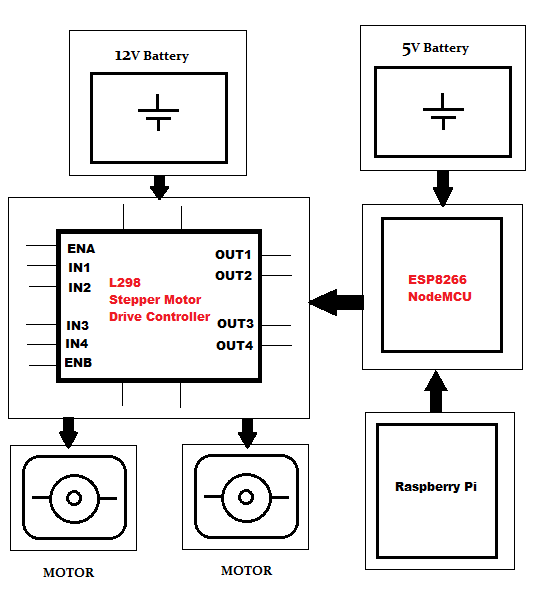
\includegraphics[width=\columnwidth]{images/FlowDiagram.png}
      \caption{Data Flow Diagram}\label{F:flow}
\end{figure}

\section{Software and Hardware Requirements}

\subsection{Software Requirement}
The Software Requirements for designing Robot car includes:
1. JDK
2. Arduino IDE
3. Raspbian Operating System

\subsubsection{JDK:Java Platform (JDK)}
The Java Development Kit (JDK) is an implementation of either one of the 
Java SE, Java EE or Java ME platforms released by Oracle Corporation in the 
form of a binary product aimed at Java developers on Solaris, Linux, Mac OS 
X or Windows. The JDK includes a private JVM and a few other resources to 
finish the recipe to a Java Application.

\subsubsection{Arduino IDE}
Arduino IDE tool. This open-source tool allows to write programs and 
uploaded into any arduino supported boards. It can be operated in two ways. 
If there is a reliable internet connection, Ardiono Web Editor (online IDE) 
can be used allowing to save the sketches to store in the cloud and having 
them available from any type of device and to have a good backup. For 
offline works, Desktop IDE can be used~\cite{arduino2015}. To program into 
esp8266 NodeMCU, Ardiono IDE is installed on Raspberry Pi to check the code 
and loads it into esp8266 board.

\subsubsection{Raspbian OS}
Raspbian is a open-source operating system based on Debian which is 
optimized for Raspberry Pi hardware. This operating system comes with 35000 
inbuilt packages, pre-compiled software for easy installation on Raspberry 
Pi.

\subsection{HARDWARE REQUIREMENT}
The Hardware components required for our project are Min 1 GB of RAM,10 GB 
HDD, Dual core processor for the machine on which development will be done, 
Robot kit, IP Camera, Bluetooth Module for developing the robot.

Hardware Requirement
\begin{itemize}
\item[a.] Raspberry Pi
\item[b.] esp8266 NodeMCU micro-controller
\item[c.] L298N Dual H-Bridge Stepper Motor Controller
\item[d.] DC power supply 12v and 5v
\item[e.] Robot Car chassis kit
\item[f.] HC-SR04 Ultrasonic Sensor
\item[g.] SG90 Servo Motor
\item[h.] Wires, Breadboard, Small PCB
\end{itemize}


\section{Basic Design of the Robot}
Robot car is built with esp8266 NodeMCU microcontroller on which programming 
code is written to control the navigation. An esp8266 is connected with two 
wheel DC motors through L298 stepper motor driver controller (pins IN1, IN2, 
IN3, IN4) which provides electric power to the motors. Wheel actuators are 
used to move robot in different directions (forward, backward, right, left 
and stop).

The movement of robot car will stop once an obstacle is detected along its 
path which can be detected by an ultrasonic sensors. Then the sensor will 
look for the best path to navigate based on the right side and left side 
distances received from the sensor.

\subsection{Ultrasonic Sensors for Obstacle Avoidance}
Ultrasonic sensors are typically used as part of computer vision, Sonar. 
These are used to provide precise and non-contact distance measurements 
in its view within a 3 centimeters to 400 centimeters range. Ultrasonic 
sensors work in any lighting condition environments, making a good 
alternative to supplement infrared object detectors.

Working Principle: The ultrasonic sensor emits a high frequency and short 
range signals. These signals travel in air at the speed of velocity of 
sound. If the signal is hit to any obstacle, then it will reflect back the 
echo signal to the sensor. A multi-vibrator is fixed to the base of an 
ultrasonic sensor. It`s the combination of a vibrator and a resonator. The 
working principle of resonator is to  deliver the  ultrasonic wave generated 
by the vibration from the vibrator. The ultrasonic sensor consists of two 
parts; the emitter which produces a 40 kHz sound wave and detector detects 
40 kHz sound wave and sends electrical signal back to the micro-
controller~\cite{ijedr2016}. The diagram in the Figure~\ref{F:usensor} shows 
the pin connectivity of ultrasonic sensor to esp8266 NodeMCU module.

\begin{figure}[htb]
	\centering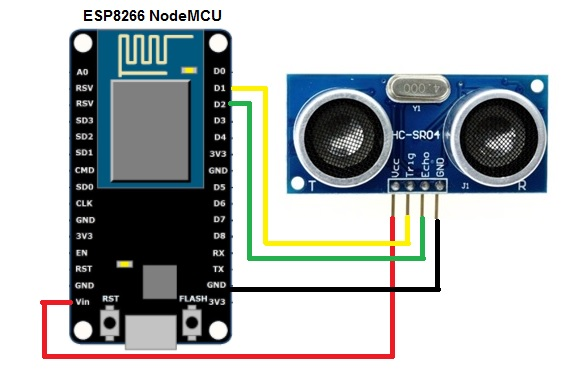
\includegraphics[width=\columnwidth]{images/Ultrasonic-sensor.jpg}
	\caption{HC-SR04 Sensor Diagram}\label{F:usensor}
%\end{figure}

%\begin{figure}
	\centering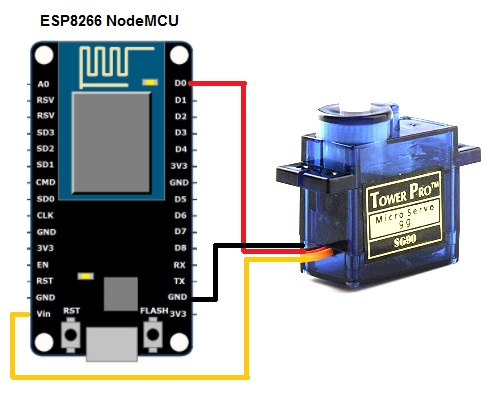
\includegraphics[width=\columnwidth]{images/SG90-servo.jpg}
	\caption{SG90 Servo Motor Diagram}\label{F:sg90}
%\end{figure}

%\begin{figure}
	\centering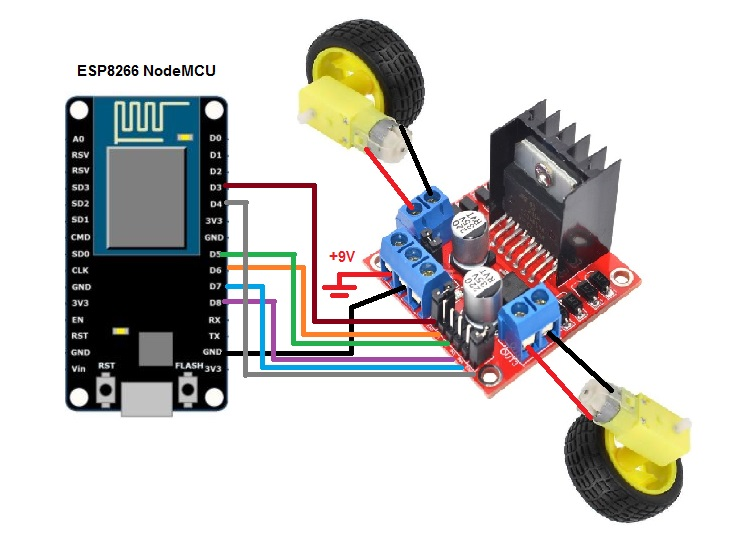
\includegraphics[width=\columnwidth]{images/L298N_Hbridge.jpg}
	\caption{L298N Dual H-bridge Stepper Motor}\label{F:stepper}
\end{figure}

\subsection{SG90 Servo Motor}
SG90 servo motor is used to control the directions of ultrasonic sensor. 
When an obstacle is detected by ultrasonic sensor, robot car will stop its 
motion and sends signal to SG90 servo motor to rotate right and left 
directions. Based on the direction ultrasonic sensor will measure the 
distance and move the robot to the direction which is longer in distance. 
The diagram in Figure~\ref{F:sg90} shows the  connectivity of servo motor to 
esp8266 NodeMCU board.

\subsection{L298N Dual H-Bridge Stepper Motor Controller}
The L298N Dual H-Bridge Motor Driver Board is cheapest, great value and can 
be used with a variety of robot controllers. A powerful L298N motor driver 
module is featured with a heavy duty heat sink. It is powerful enough to 
drive motors from 5-35V at up to 2A peak~\cite{bananarobotics2013}.

DC motor wheels of Robot is powered using L298N stepper motor which is a 
typical robot motor driver. A 9v battery pack is connected to the stepper 
motor controller. The diagram in the Figure~\ref{F:stepper} shows the pin 
connectivity of stepper motor controller with the wheel DC motors and 
esp8266 NodeMCU board.

\subsubsection{Connectivity to DC motors and esp8266 NodeMCU}
For the connectivity if DC motors to esp8266 NodeMCU board, robot wheel 
DC motors are to be attached to the MotorA and MotorB terminal screws 
of stepper motor controller. In the Table~\ref{T:pinlayout} shows the 
GPIO pin connectivity of esp8266 board to stepper motor controller pins.

\begin{table}[htb]
\caption{esp8266 GPIO to stepper motor pin connections}\label{T:pinlayout}
\begin{tabular}{lll}
Actuator & GPIO Pin & L298N Pin \\
\hline
    RightMotorForward & GPIO12 & IN1 \\
    RightMotorBackward & GPIO14 & IN2 \\
    LeftMotorForward & GPIO15 & IN3 \\
    LeftMotorBackward & GPIO13 & IN4 \\
    RightMotorENB & GPIO0 & ENA \\
    LeftMotorENB & GPIO2 & ENB \\
\end{tabular}
\end{table}

The following Table~\ref{T:gpiooutput} show the programming of GPIO pin 
outputs for the robot car to move in corresponding directions. When the pin 
status shows 1, it means that GPIO output of that pin will have triggered 
voltage of 5volts. When the pin status shows 0, then there won't be any 
voltage triggered.

\begin{table}[htb]
\caption{GPIO pin output for movement of robot car}\label{T:gpiooutput}
\begin{tabular}{lllll}
Movement & Pin 12 & Pin 14 & Pin 15 & Pin 13 \\
\hline
Forward & 1 & 0 & 1 & 0 \\ 
Backward & 0 & 1 & 0 & 1 \\
Left & 1 & 0 & 0 & 1 \\
Right & 0 & 1 & 1 & 0 \\
Stop  & 0 & 0 & 0 & 0 \\
\end{tabular}
\end{table}

\subsection{Arduino IDE setup}
\subsubsection{Steps:}
The following steps shows how to configure Ardiono IDE setup in raspberry pi 
and to install esp8266 community build on the Ardiono IDE to support esp8266 
NodeMCU board.

\begin{itemize}

\item Install Arduino IDE on Raspberry Pi
\item Once installed, lauch Ardiono IDE and select Tools
\item From the dropdown, select Board:  and then select Boards Manager
\item Navigate to esp8266 by esp8266 community and install the
  software for Arduino.
\item Once the software is installed, goto Tools and select Board:
  ``NodeMCU 1.0 (ESP-12E Module)''
\item Choose CPU Frequency as 80 MHz
\item Select Upload Speed to 115200
\item Select appropriate port to which esp8266 is connected to
  Raspberry Pi for the first time.

\end{itemize}
Figure~\ref{F:arduino} shows the configuration setup for esp8266 NodeMCU 
board in Arduino IDE tool.
\begin{figure}
	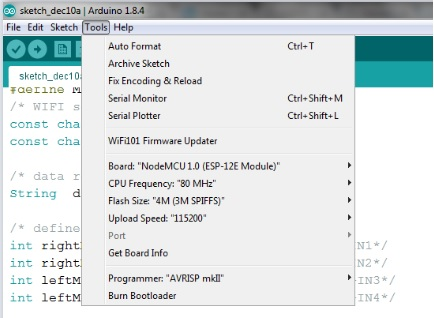
\includegraphics[width=1.0\columnwidth]{images/Arduino-settings.jpg}
	\caption{Arduino IDE configuration setup}\label{F:arduino}
\end{figure}

\section{Code}
Code for obstacle avoidance robot car is ``Robot-Obstacle-Avoidance.ino'' 
and is placed in ``code'' directory. C+ programming is being used to write 
code for the robot car. Copy this code to Arduino IDE tool which is 
installed on Raspberry Pi and push the code to esp8266 NodeMCU using wifi or 
USB cable.

\section{Working Images}
In the Figure~\ref{F:topview}, top view construction of designed robot car 
is displayed with all the connections being done. Side view of the car can 
be seen in Figure~\ref{F:sideview} and the front view in 
Figure~\ref{F:frontview}
\begin{figure}[htb]
	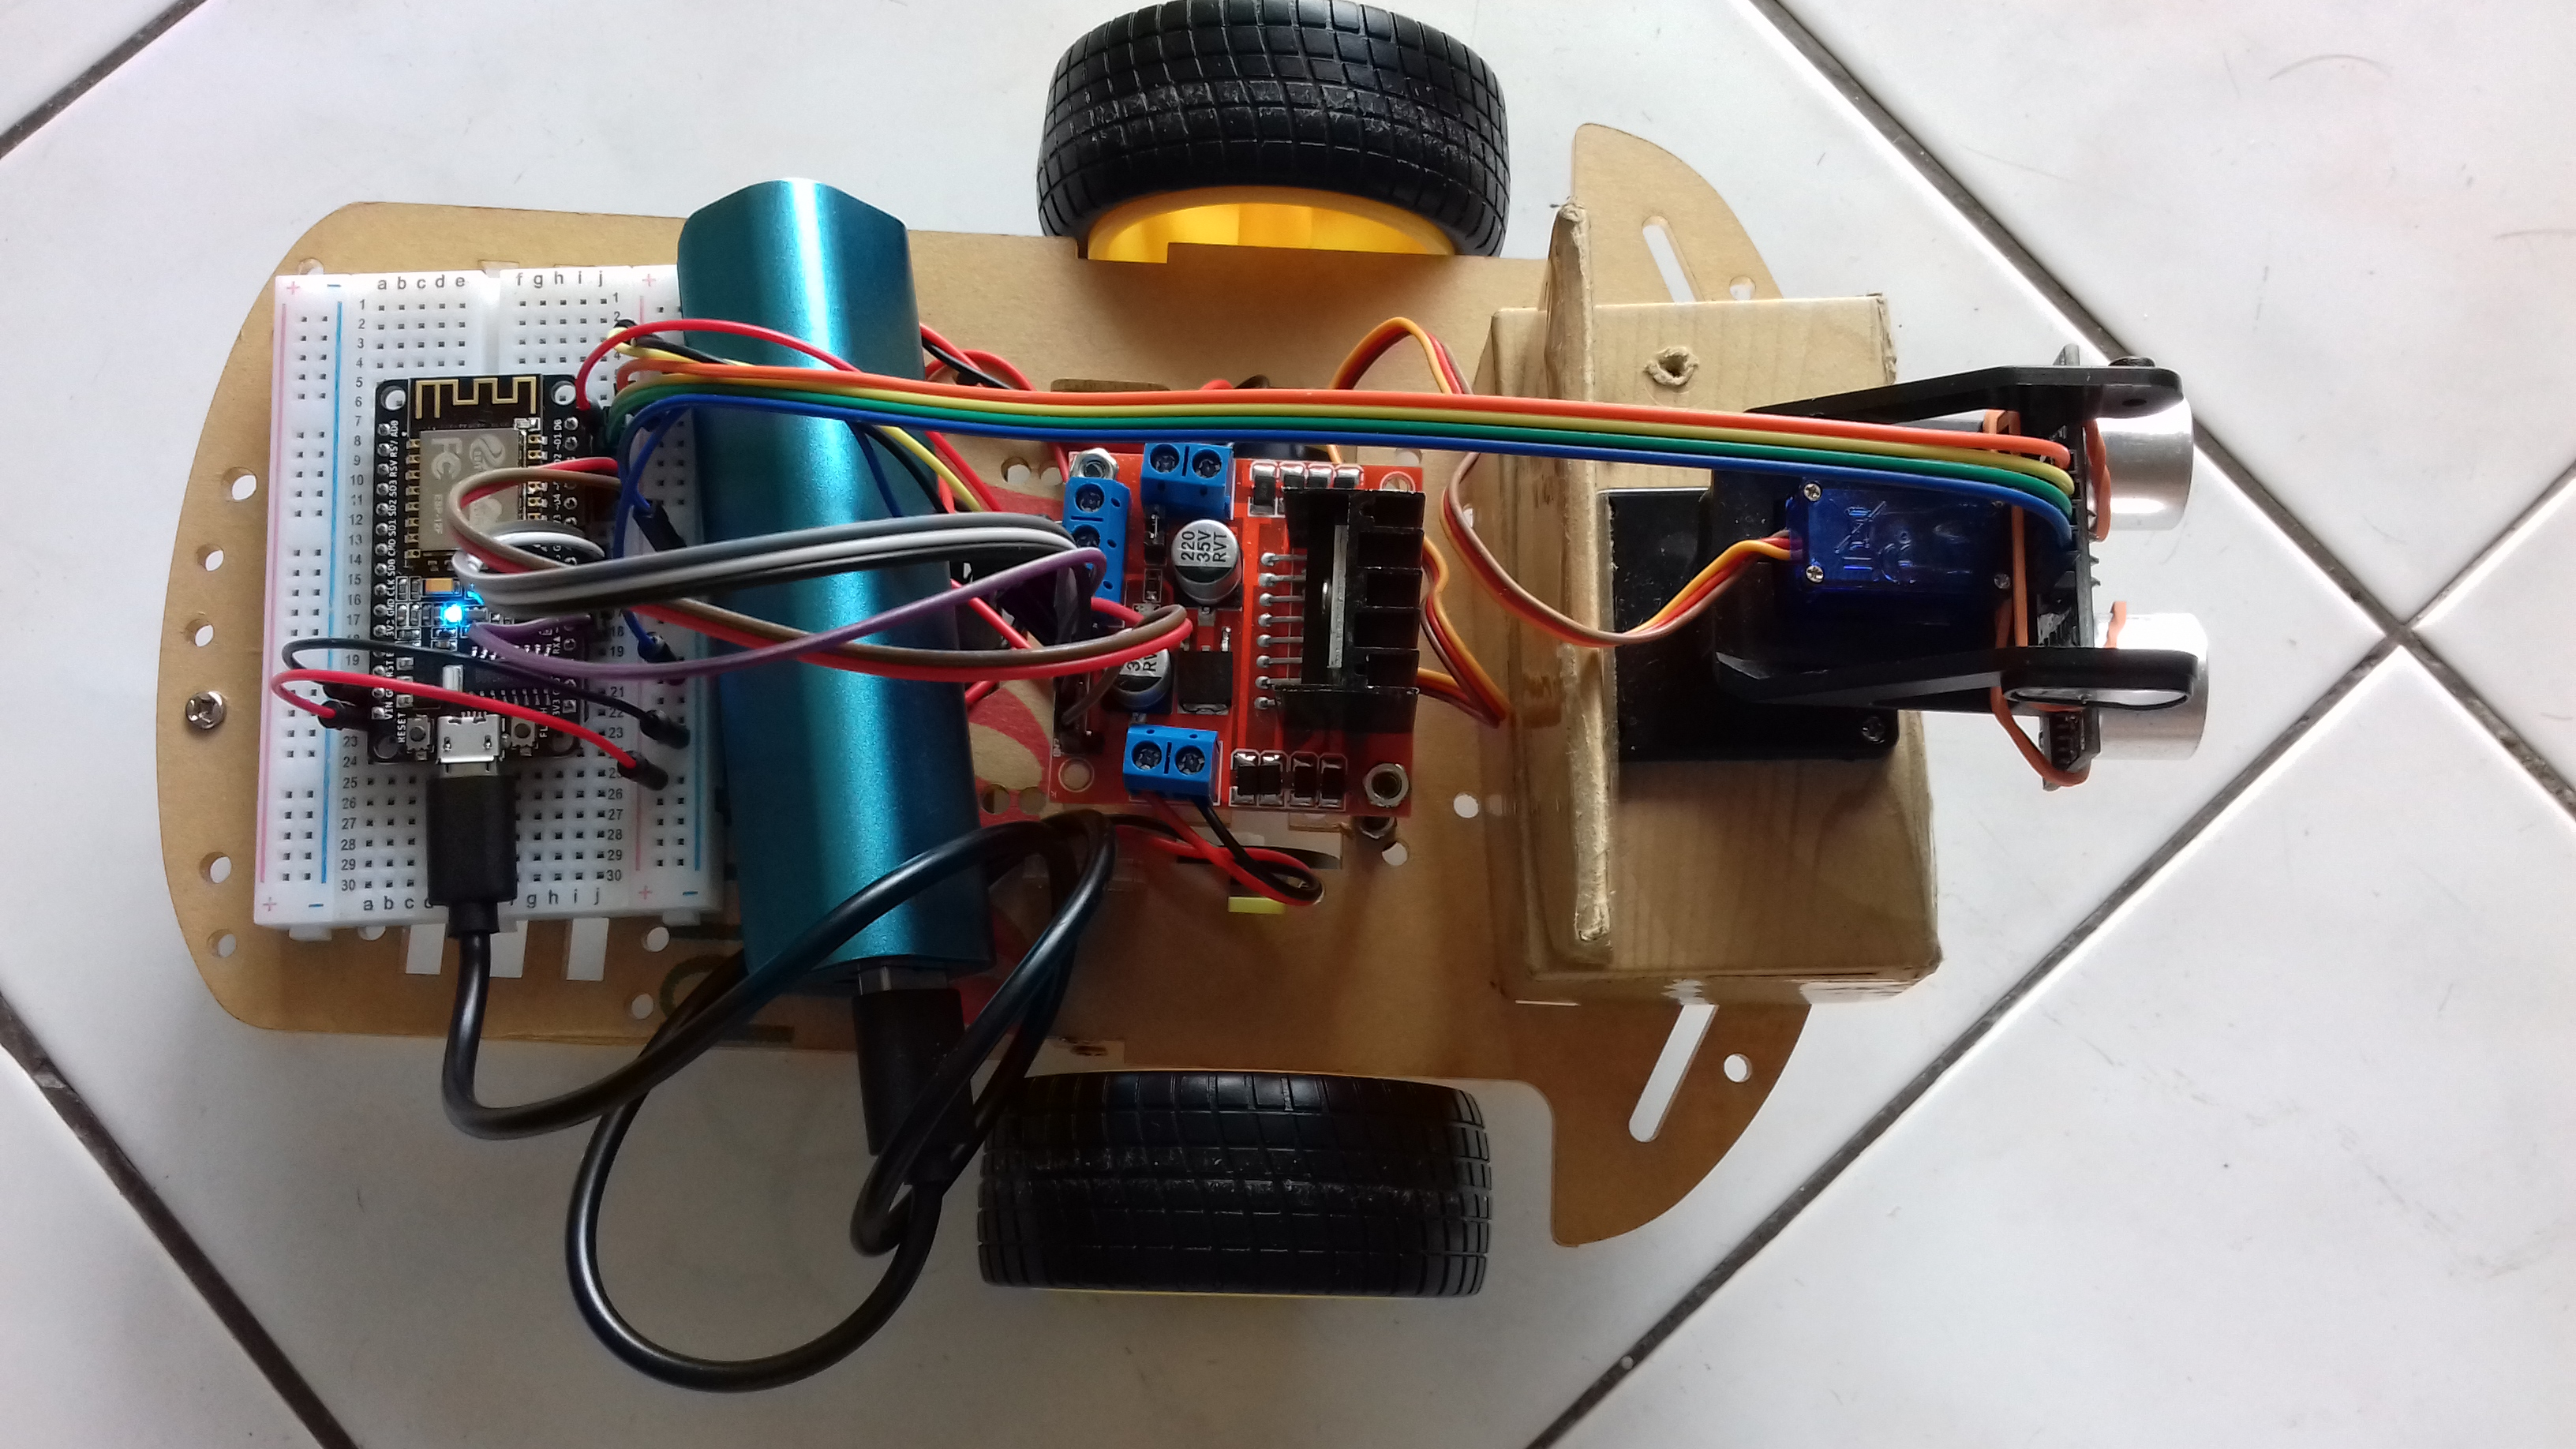
\includegraphics[width=1.0\columnwidth]{images/Top-view.jpg}
	\caption{Top View of Robot Car}\label{F:topview}
%\end{figure}

%\begin{figure}
	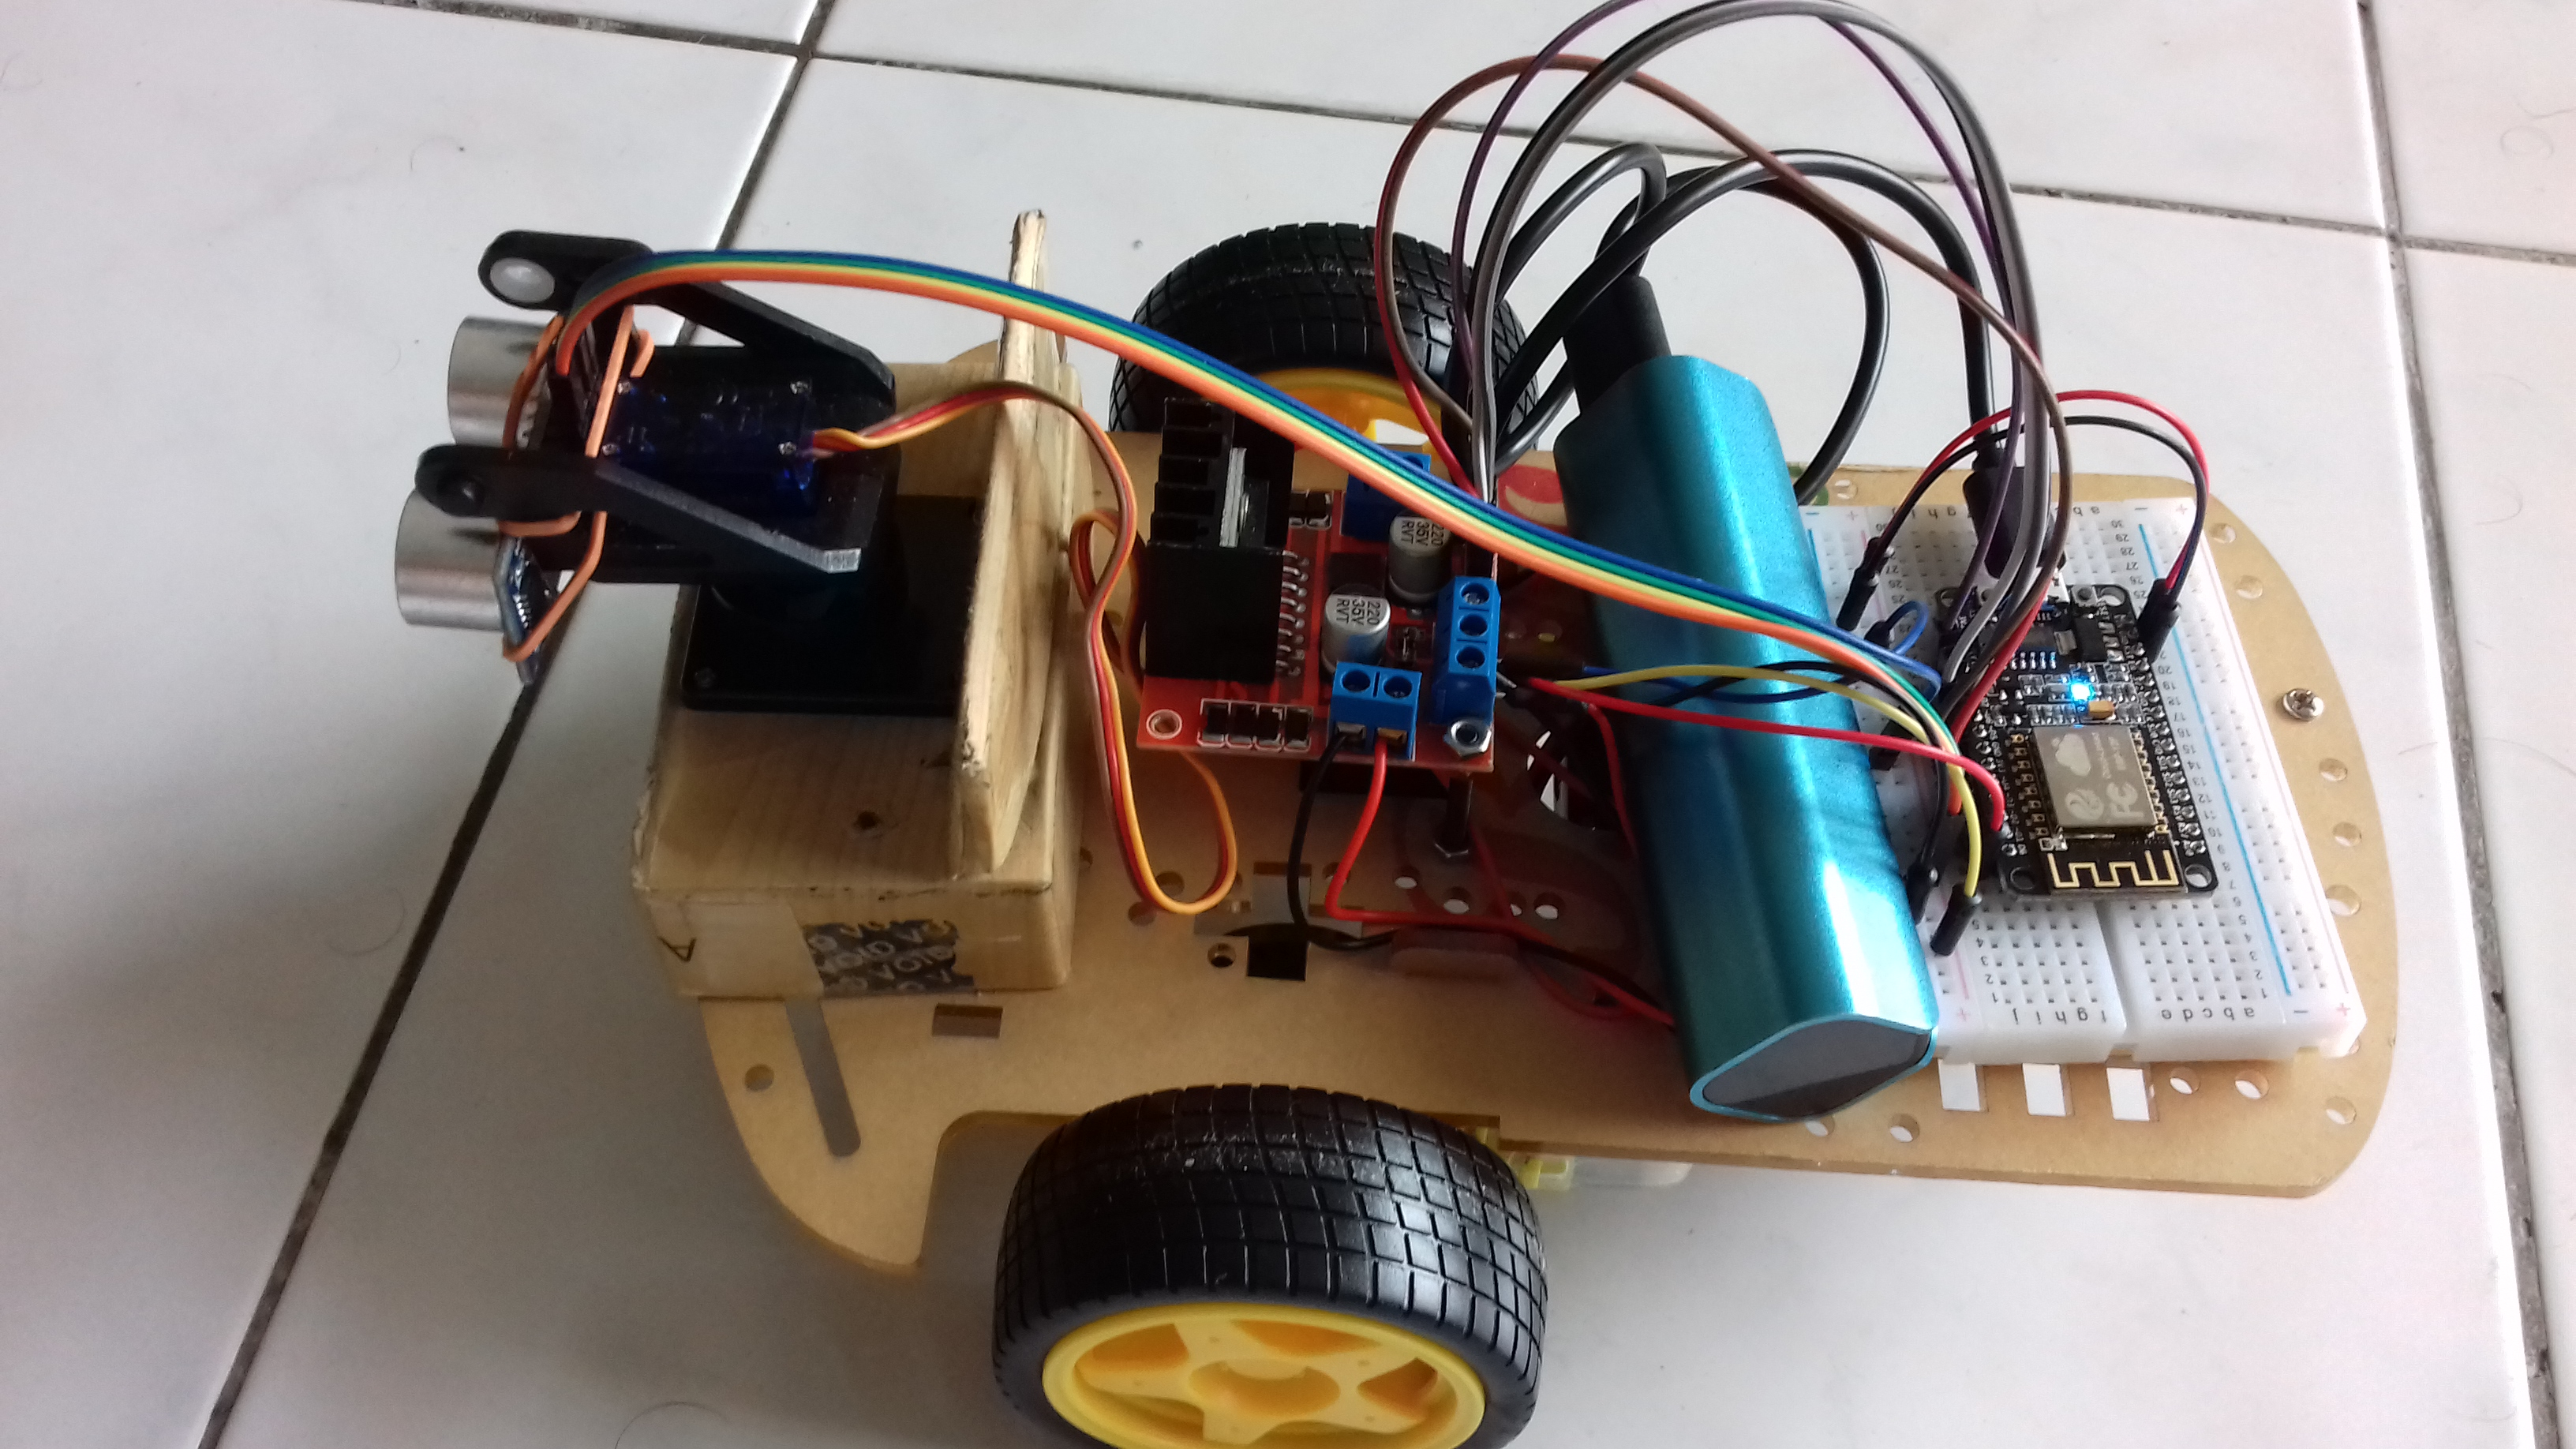
\includegraphics[width=1.0\columnwidth]{images/Side-view2.jpg}
	\caption{Side view of Robot Car}\label{F:sideview}
%\end{figure}

%\begin{figure}
	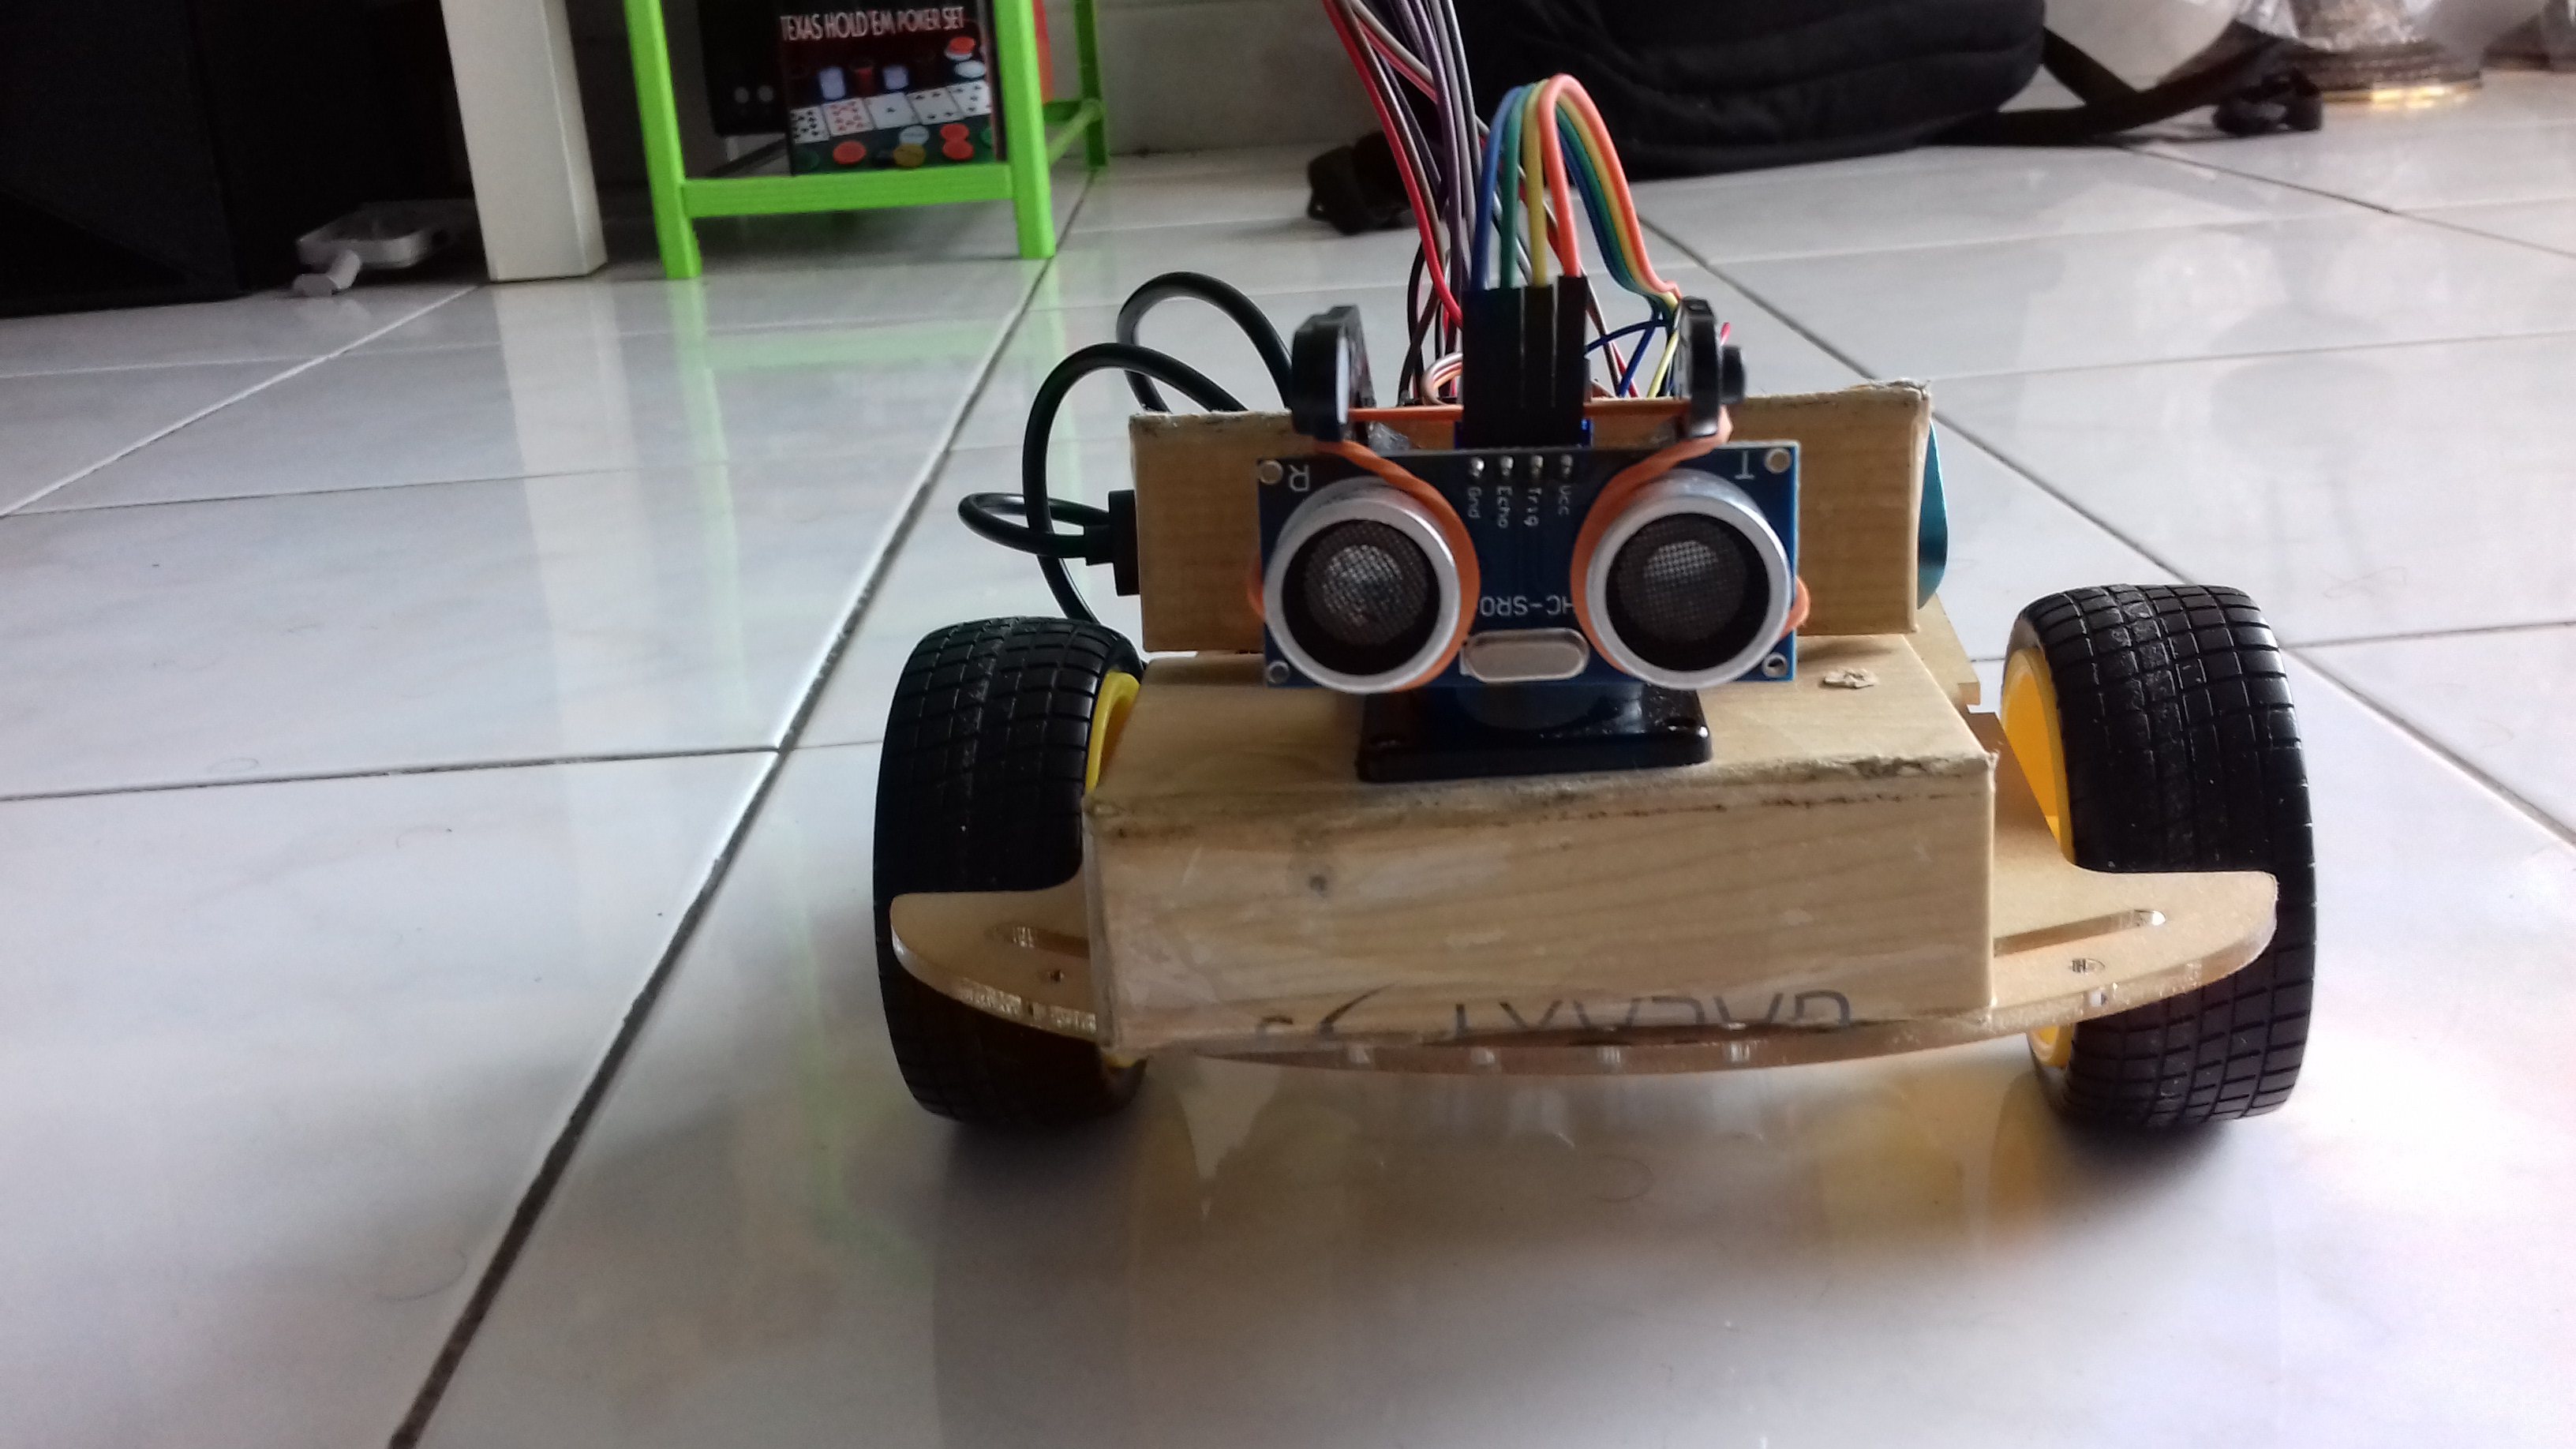
\includegraphics[width=1.0\columnwidth]{images/Front-view.jpg}
	\caption{Front View of Robot Car}\label{F:frontview}
\end{figure}

\section{Applications}
\begin{itemize}
    \item[1.] Scientific
    \item[2.] Space Probes
    \item[3.] Submarines
    \item[4.] Military and Law Enforcement
    \item[5.] Recreation and Hobby
\end{itemize}

\section{Conclusion}
In these modern days, long distance communication is a crucial theory of 
controlling things from internet and this leads a for a vast application 
areas. Obstacle avoidance robot can be controlled by wifi which can track 
the obstacles along its path way and can be easily controlled remotely.

\begin{acks}

The authors would like to thank Dr Gregor von Laszewski for his support 
and suggestions in writing this paper.

\end{acks}

\bibliographystyle{ACM-Reference-Format}
\bibliography{report} 

\appendix

\section{Code}

In this section we present the code that is organized as follows:

\VerbatimInput{code/Robot-Obstacle-Avoidance.ino}
